\documentclass[oneside, final, 14pt]{extreport}
\usepackage[utf8]{inputenc}
\usepackage[russian]{babel}
\usepackage{vmargin}
\setpapersize{A4}
\setmarginsrb{2cm}{1cm}{1cm}{1cm}{0pt}{0mm}{0pt}{13mm}
\usepackage{indentfirst}
\usepackage{amsmath}
\usepackage{graphicx}
\usepackage{wrapfig}
\sloppy

\begin{document}

\setcounter{chapter}{3}
\chapter{Анализ звука}
\section{Анализ звука: цели, задачи и инструменты Adobe Audition}
Цель анализа звуковой информации: оценить ее пригодность и наметить стратегию обработки, позволяющую устранить имеющиеся недостатки.

В нашем распоряжении имеются следующие средства анализа:
\begin{itemize}
\item мониторинг (прослушивание) записи;
\item качественный визуальный анализ сигналограммы и уровня записанного аудиосигнала;
\item статистический амплитудный анализ сигналограммы;
\item анализ спектрограммы;
\item анализ амплитудно-частотного спектра;
\item анализ фазы сигнала.
\end{itemize}

Рассмотрим каждое из средств анализа подробнее.
\subsection{Мониторинг}
Прежде всего, записанный звук следует внимательно и многократно прослушать. Цель такого прослушивания состоит в том, чтобы оценить пригодность записи для дальнейшей обработки, а также отбраковать фрагменты, содержащие грубые ошибки.

Если делалась многократная запись одного и того же материала, то на этом этапе следует выбрать дубли с самым высоким качеством записи. Если нет ни одного дубля, полностью от начала до конца пригодного для дальнейшей обработки, то можно выбрать несколько дублей, и в дальнейшем следует смонтировать необходимую запись из лучших фрагментов разных дублей.

При мониторинге следует обращать внимание на следующие моменты:
\begin{itemize}
\item наличие постоянных фоновых шумов;
\item наличие щелчков;
\item наличие искажений тембра. 
\end{itemize}

Этапы анализа звука будут продемонстрированы на основе примера из книги~[1]. Файл \textit{track 01.wav}~--- часть проекта, целью которого является запись короткого видеоролика, содержащего звуковое сопровождение. Ролик посвящен аппаратуре, необходимой в домашней звуковой студии. Съемки и звукозапись проводились на базе питерского магазина \textit{MusicLand}. В качестве диктора и ведущего выступает его директор и давний участник проекта "<Музыкальный компьютер"> Вадим Лукин.

Рассмотрим процесс мониторинга записи на примере файла \textit{track 01.wav}. Файл создавался без прерываний записи, и дубли идут один за одним. В данном файле хранятся пять дублей записи одной и той же фразы. 

Итогом первого этапа анализа можно считать следующие выводы.
\begin{itemize}
\item Первый дубль (фрагмент в интервале от 0:00 до 0:34) непригоден для дальнейшего использования из-за того, что в голосе человека, читавшего текст, иногда слышен хрип. В дальнейшем этот фрагмент волновой формы целесообразно вырезать, чтобы сократить размер файла и время его обработки.
\item Второй дубль (от 0:37 до 1:13) записан с перегрузкой микрофона. Человек, читающий текст, в ряде мест излишне акцентировал свою речь. Поэтому, хотя большинство максимумов волновой формы находится примерно на уровне $-6$ дБ, встречаются отдельные выбросы, достигающие $0$ дБ. Имеется также переполнение разрядной сетки АЦП. Дубль № 2 пока можно сохранить на тот случай, если в дальнейшем потребуется скомбинировать отдельные фрагменты, взятые из разных дублей.
\item Третий дубль (от 1:16 до 1:49) содержит меньше материала с клипированием, чем дубль № 2, однако в нем нас не устроила интонация диктора, который к моменту записи этого дубля уже заметно устал, а его голос сник.
\item Четвертый дубль (от 1:51 до 2:25), записанный после небольшой паузы, во время которой диктор отдохнул и осмыслил свою задачу, следует считать  предпочтительным,  хотя  видно,  что  в  нем тоже  есть  отдельная клипированные отсчеты. 
\item Пятый дубль (от 2:27 до 3:01) записан без клипирования. Уровень записи был уменьшен,а микрофон отодвинут подальше от диктора. Удаление микрофона от источника звука в свою очередь вызвало изменение звукового плана: на фоне несколько ослабленного прямого звука стал заметнее звук, отраженный стенами помещения и предметами, находящимися в нем. Иными словами, стала проявлять себя реверберация, в данном случае нежелательная, т. к. запись велась в не совсем подходящем для этой цели помещении, и такая реверберация, не украшая звук, снизила разборчивость речи. Тем не менее, и этот дубль в дальнейшем может быть выбран в качестве основного. Решение о том, какой дубль (№ 4 или № 5) следует использовать, целесообразно принимать на последнем этапе.
\end{itemize}

\subsection{Визуальный анализ волновой формы}
При визуальном анализе сигналограммы следует обратить на следующее:
\begin{itemize}
\item максимальный уровень громкости сигнала;
\item как часто достигается уровень громкости $0$~dBFS;
\item присутствуют ли в записи постоянные фоновые шумы;
\item присутствуют ли в записи щелчки;
\item динамика звука (переходы от тихих звуков к громким).
\end{itemize}

\begin{figure}[h]
\centering
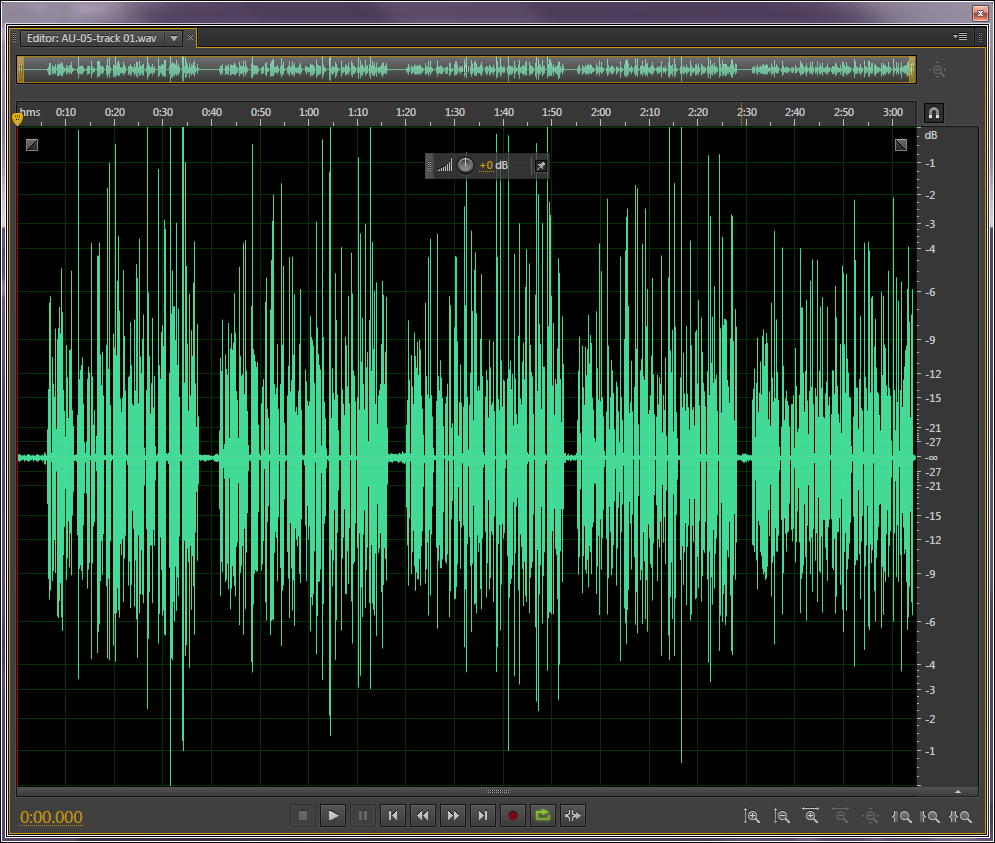
\includegraphics[width=0.75\textwidth]{pic-fivedoubles-01}
\caption{Сигналограмма пяти дублей}
\label{pic-fivedoubles-01}
\end{figure}

\subsection{Статистический амплитудный анализ}
Результат амплитудного анализа будет использоваться при решении вопроса о целесообразности борьбы с некоторыми шумами, искажениями, и при выборе параметров динамической обработки записанного сигнала.

Сбор статистической информации о волновой форме осуществляется с помощью окна \textit{Amplitude Statistics}, открываемого командой \textit{Window > Amplitude Statistics}.

Окно содержит три вкладки: 
\begin{itemize}
\item \textit{General}~--- статистическая информация о параметрах волновой формы;
\item \textit{RMS Histogram}~--- гистограмма (распределение значений) отсчетов волновой формы;
\item \textit{RMS Settings}~--- настройки для расчета гистограммы.
\end{itemize}

Вкладка General содержит статистическую информацию или о выделенном звуковом фрагменте, или обо всей волновой форме.

\begin{figure}[h]
\centering
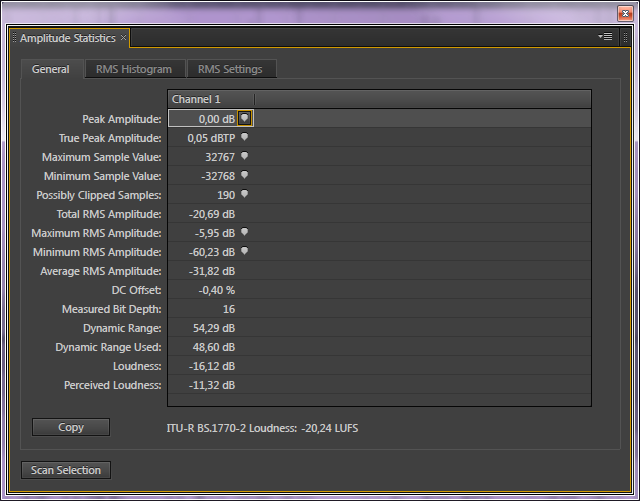
\includegraphics[width=0.75\textwidth]{pic-analis-01}
\caption{Вкладка \textit{General} окна \textit{Amplitude Statistics}}
\label{pic-analis-01}
\end{figure}

В столбцах для стереоканалов (или в единственном столбце в
случае монофонического сигнала) представлена статистическая информация, наиболее важными из которых являются следующие:
\begin{itemize}
\item \textit{Peak Amplitude}~--- пиковая амплитуда сигнала;
\item \textit{Possibly Clipped Samples}~--- количество отсчетов, имеющих
уровень 0 \textit{dBFS} (клиппированных отсчетов);
\item \textit{DC Offset}~--- уровень постоянной составляющей в выделенном фрагменте волновой формы;
\item \textit{Minimum RMS Power}~--- минимальное значение среднеквадратичной мощности;
\item \textit{Average RMS Power}~--- среднее значение среднеквадратичной мощности;
\item \textit{Dynamic Range}~--- динамический диапазон сигнала;
\item \textit{Dynamic Range Uses}~--- использованный динамический диапазон;
\item \textit{Loudness}~--- громкость;
\item \textit{Perceived Loudness}~--- воспринимаемая громкость (с учетом чувствительности слуха человека);
\end{itemize}

Параметр \textit{Peak Amplitude}~--- это максимальный уровень громкости звукового отсчета в выделенном фрагменте. Значение пиковой амплитуды определяет, на какую величину можно произвести усиление амплитуды без искажений. Например, если пиковая амплитуда равна $-3.1$ dBFS, то можно увеличить амплитуду сигнала на $+3.1$ дБ.

По значению пиковой амплитуды нельзя сравнивать громкость
двух аудио фрагментов, так как этот параметр не дает информации о
средней громкости на протяжении всего отрезка времени.

При расчете громкости сигнала используется следующий метод:
\begin{enumerate}
\item Вся временная ось разбивается на небольшие интервалы постоянной длины, которое задается в поле \textit{Window Width <...> ms}.
\item В каждом интервале сигнал сравнивается с эталонной волной (либо синусоидальной, либо состоящей из прямоугольных импульсов, что задается в \textit{RMS Settings}, громкость которой считается равной 0dB).
\item Осуществляется расчет минимальной, максимальной (\textit{Minimum/Maximum RMS Power}), средней и суммарной громкости (\textit{Average RMS Power}, \textit{Total RMS Power}) на основе значений, рассчитанных для всех интервалов.
\end{enumerate}

Рассмотрим статистические сведения файла \textit{track 01.wav}.
\begin{itemize}
\item \textit{Peak Amplitude}: $0.00$  dB
\item \textit{Max Sample Value}: $ 32 767$
\item \textit{Min Sample Value}: $-32 768$
\item \textit{Possibly Clipped Samples}:	$190$
\item \textit{Total RMS Amplitude}: $-20.69$ dB
\item \textit{Maximum RMS Amplitude}: $-5.95$ dB
\item \textit{Minimum RMS Amplitude}: $-60.23$ dB
\item \textit{Average RMS  Power}: $-31.82$ dB
\item \textit{DC Offset}: $-0.40$
\item \textit{Measured Bit Depth}: $16$ Bits
\item \textit{Loudness}: $-16.12$ dB
\item \textit{Percieved Loudness}: $-11.32$ dB
\end{itemize}

Обратим внимание на параметры:
\begin{itemize}
\item \textit{Possibly Clipped} = $190$~--- имеется 190 клиппированных отсчетов, они дают неприятный эффект "<захлебывания">, и их в дальнейшем предстоит обработать с целью восстановления формы сигнала на клиппированных участках;
\item \textit{DC Offset} = $-0.40\%$~--- в волновой форме присутствует небольшая постоянная составляющая, что при монтаже может вызвать щелчки в местах склейки и разрезания фрагментов.
\end{itemize}

\textit{Клиппирование}~--- это искажение, возникающее из-за неправильной регулировки уровня записываемого сигнала или из-за его случайного увеличения во время записи, приведшее к переполнению разрядной сетки аналого-цифрового преобразователя (см. рис. \ref{pic-clipping-01}). Клиппирование~--- искажение, крайне неприятное для слуха.

\begin{figure}[h]
\centering
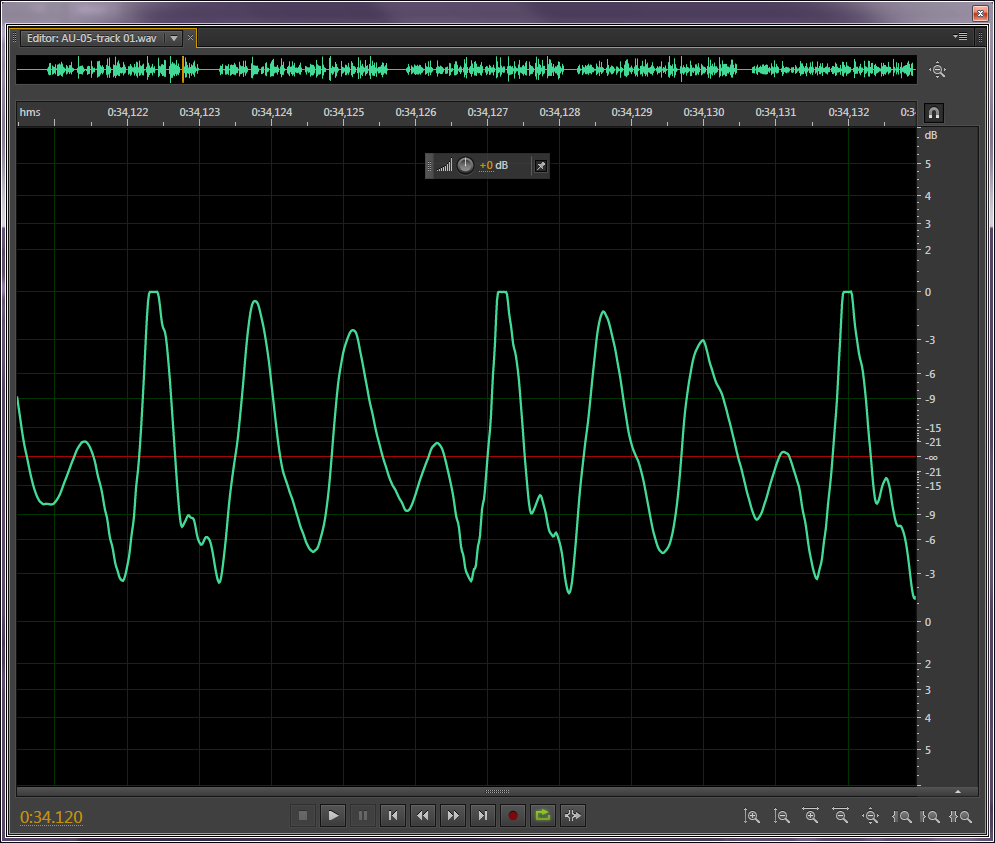
\includegraphics[width=0.5\textwidth]{pic-clipping-01}
\caption{Пример клипирования}
\label{pic-clipping-01}
\end{figure}

Значение \textit{Possibly Clipped Samples}~--- это количество клиппированных отсчетов, то есть отсчетов, имеющих уровень 0 dBFS. При редактировании \textit{Adobe Audition} допускает превышение уровня громкости в 0 dBFS. При сохранении эти отчеты станут клиппированными. Если количество клиппированных отсчетов сигнала невелико (не превышает несколько десятков), то от клиппирования можно будет в дальнейшем избавиться при помощи соответствующей обработки, в противном случаем материал следует переписать его заново. 

Параметр \textit{DC Offset}~--- уровень постоянной составляющей в выделенном фрагменте волновой формы. Если уровень постоянной составляющей равен 0\%, то колебания волновой формы происходят относительно линии нулевой громкости. Это нормальное значение параметра \textit{DC Offset}. (см. рис. \ref{pic-dcoffset-01})

\begin{figure}[h!]
\centering
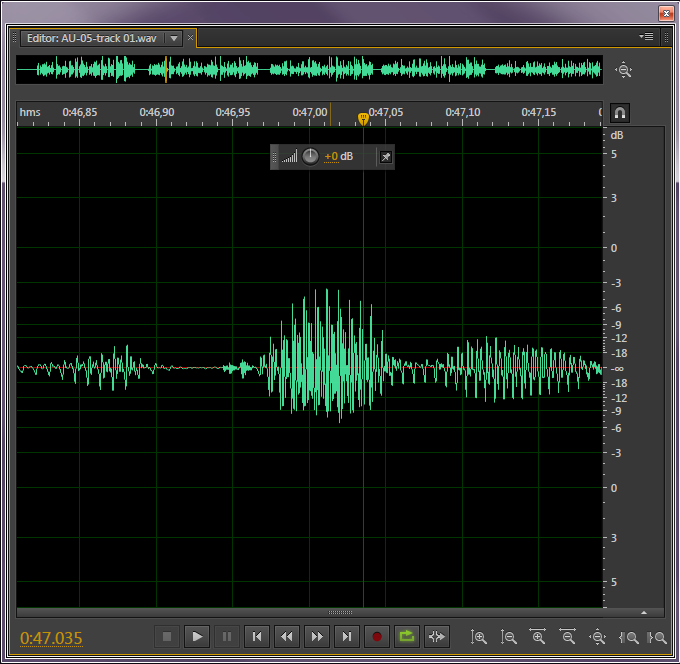
\includegraphics[width=0.5\textwidth]{pic-dcoffset-01}
\caption{Пример записи с уровнем постоянной составляющей 0\%}
\label{pic-dcoffset-01}
\end{figure}
Если уровень постоянной составляющей отличен он нуля, то колебания происходят относительно линии, отличной от линии нулевой громкости (см. рис. \ref{pic-dcoffset-02}).

\begin{figure}[h!]
\centering
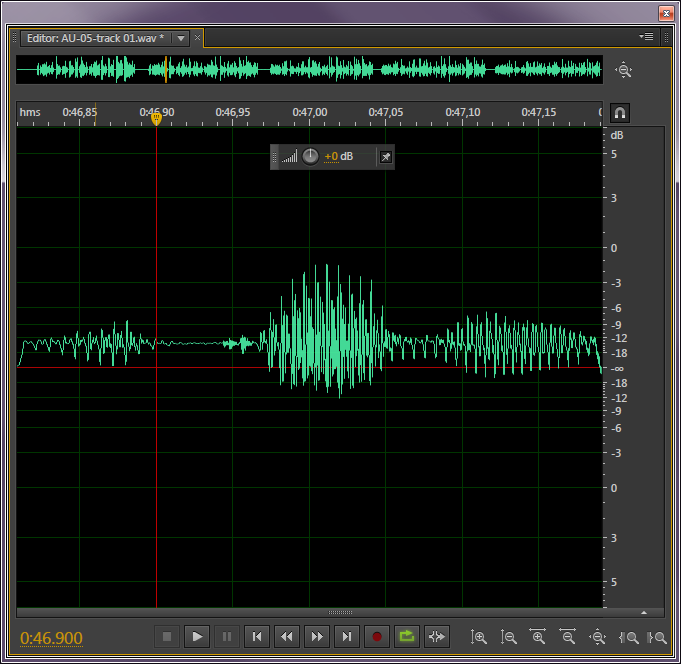
\includegraphics[width=0.5\textwidth]{pic-dcoffset-02}
\caption{Пример записи с уровнем постоянной составляющей 20\%}
\label{pic-dcoffset-02}
\end{figure}

Значение данного параметра не влияет на восприятие записи, однако, при обработке необходимо будет избавиться от постоянной составляющей, так как наличие постоянной составляющей уменьшает динамический диапазон звука. Кроме того, при монтаже звуков с разными значениями данного параметра будут слышны щелчки в местах
монтажа.

Параметр \textit{Minimum RMS Power}~--- это минимальное значение среднеквадратичной мощности. Если величина данного параметра ниже -85 dBFS, то это говорит о наличии в записи фрагментов абсолютной тишины. Чем больше величина данного параметра, тем громче фоновый шум в записи.

Громкость следует оценивать по параметрам \textit{Loudness} и \textit{Perceived Loudness}. Именно по данным параметрам, а не по пиковой амплитуде, нужно сравнивать громкость различных записей.

Выделив поочередно каждый из пяти дублей, и проанализировав выделенные участки волновой формы, вы можете сравнить основные их параметры.

\begin{table}[ht]
  \caption{Результат сравнения пяти дублей}
  \begin{center}
  \begin{tabular}{|l|c|c|c|c|c|}
    \hline Параметр 				& Дубль 1 	& Дубль 2 	& Дубль 3 	& Дубль 4 	& Дубль 5\\
    \hline Possible Clipped Samples & 108 		& 39 		& 4 		& 39 		& 0\\
    \hline Minimum RMS Amplitude 	& -57.77	& -56.76    & -60.22	& -60.05	& -56.58\\    
    \hline Loudness 				& -13.69	& -15.18	& -15.09	& -12.83	& -17.13\\    
    \hline 
  \end{tabular}
  \end{center}  
  \label{table-fivedoubles-01}
\end{table}

Сравнение соответствующих значений параметров убеждает в том, что по количеству клипированных отсчетов (\textit{Possibly Clipped}) выигрывают дубли № 3 и № 5. Дубль № 3, вероятно, наименее шумный (косвенно на это указывает наименьшее значение \textit{Minimum RMS Amplitude}). Самый "<тихий"> дубль № 3 (\textit{Loudness}), а самый "<громкий">~--- дубль № 1, но он же и наиболее подвержен клипированию (\textit{Possibly Clipped}).

Значение параметра \textit{Loudness} для всех дублей мало (порядка $-20$ дБ). Речь будет звучать очень тихо по сравнению, например, с музыкой, наложенной поверх речи.

\subsection{Гистограмма}
\textit{Гистограмма}~--- широко распространенная форма представления информации о каком-либо случайном процессе. Гистограмма представляет собой графическое изображение зависимости частоты попадания элементов выборки от соответствующего интервала группировки.

В данном случае гистограмма представляет собой изображение зависимости количества отсчетов, мощность которых попадает в заданный интервал, от величины громкости в децибелах.

\begin{figure}[h!]
\centering
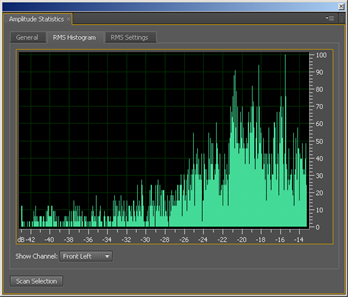
\includegraphics[width=0.5\textwidth]{pic-histogram-01}
\caption{Пример гистограммы в окне Amplitude Statistics}
\label{pic-histogram-01}
\end{figure}

\begin{figure}[h!]
\centering
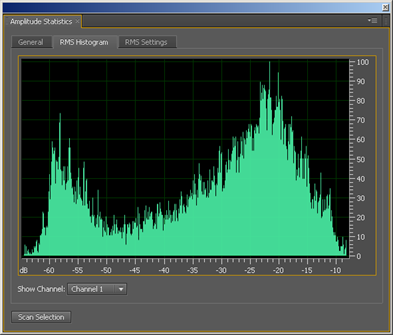
\includegraphics[width=0.5\textwidth]{pic-histogram-02}
\caption{Пример гистограммы сигнала с фоновым шумом}
\label{pic-histogram-02}
\end{figure}

На основе анализа формы гистограммы можно получить следующую
информацию:
\begin{itemize}
\item допустимый уровень порога при компрессии;
\item уровень фоновых шумов;
\item уровень ограничения для динамической обработки.
\end{itemize}

Компрессия сигнала должна осуществляться с порогом, не превышающим первый справа максимум (на рис. \ref{pic-histogram-02} это значение около $-20$~dbFS), в противном случае в процессе компрессии возникнут значительные искажения.

Если гистограмма ведет себя монотонно (рис. \ref{pic-histogram-01}), то либо в записи не присутствуют фоновые шумы, либо по громкости они неотличимы от полезного сигнала. Если гистограмма ведет себя немонотонно (рис. \ref{pic-histogram-02}), то левая часть~--- это шумы, правая~--- полезный сигнал. Для дальнейшей обработке необходимо запомнить границу шума, в данном случае это $-45$ dBFS.

Правая часть гистограммы содержит информацию о самых громких отчетах. Как правило, число таких отчетов невелико, и при динамической обработке они ограничиваются лимитером. По гистограмме следует определить примерную границу для лимитера. Для гистограммы на рисунке  \ref{pic-histogram-02} этот уровень $-10$ dBFS.

\subsection{Визуальный анализ спектрограммы}
Команда \textit{View > Show Spectral Frequency Display} включает режим отображения спектрограммы сигнала в виде градаций яркости и цвета. По горизонтальной оси отложено время, по вертикальной~--– частота. Цвет и яркость точки зависят от уровня спектральной составляющей в анализируемом сигнале на той или иной частоте (чем ярче~--- тем выше уровень). По умолчанию уровень тишины соответствует черному цвету, по мере увеличения громкости появляется красный цвет, а максимальный уровень отображается белым цветом.

\begin{figure}[h!]
\centering
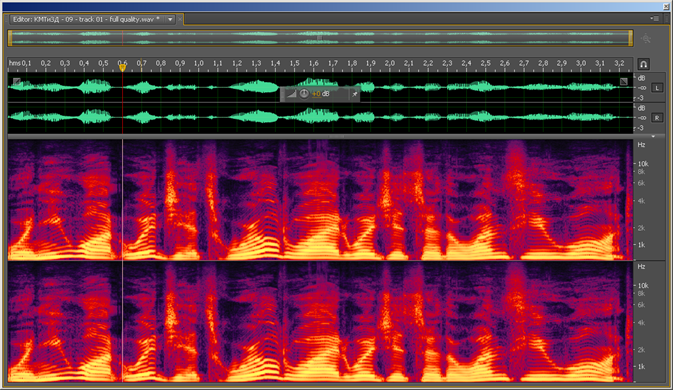
\includegraphics[width=0.95\textwidth]{pic-spectrogram-01}
\caption{Пример спектрограммы сигнала}
\label{pic-spectrogram-01}
\end{figure}

На рис. \ref{pic-spectrogram-01} представлена спектрограмма сигнала дикторского текста. Области с относительно широким спектром соответствуют словам, с узким~--- паузам между ними. Области с ярко выраженными дискретными максимумами амплитуд соответствуют гласным звукам.

Просмотр сигнала в режиме \textit{Spectral Frequency Display} позволяет визуально определить шумы или отдельные искажения, такие как: 
\begin{itemize}
\item низкочастотный гул (рис. \ref{pic-spectrogram-02}, А );
\item щелчок (рис. \ref{pic-spectrogram-02}, B);
\item высокочастотное шипение (рис. \ref{pic-spectrogram-02}, C).
\end{itemize}

\begin{figure}[h!]
\centering
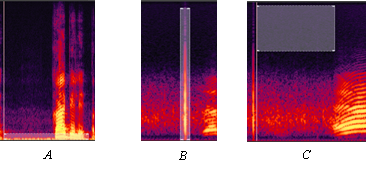
\includegraphics[width=0.75\textwidth]{pic-spectrogram-02}
\caption{Пример спектрограммы сигнала с различными шумами}
\label{pic-spectrogram-02}
\end{figure}

Щелчки и хлопки наиболее часто присутствуют на записях, которые являются результатом оцифровки виниловых пластинок, но могут также появляться при некоторых ошибках цифровой обработки сигнала, в том числе при оцифровке в случае нехватки размера буфера АЦП, в случае монтажа сигнала с разными уровнями постоянной составляющей.
Звуки размыкания губ и цокание языком также попадают в эту категорию. Данные короткие импульсные шумы отображаются на спектрограмме в виде ярких коротких по времени вертикальных линий. Чем сильнее щелчок, тем более яркой будет линия. 

При просмотре сигналограммы можно обнаружить наличие тональных шумов (шумов на постоянной дискретной частоте). В окне сигналограммы тональные шумы отображаются в виде отдельных горизонтальных линий на протяжении всего времени (рис. \ref{pic-spectrogram-03}, частота~--- 16 кГц). Тональные шумы могут возникать по разным причинам:
\begin{itemize}
\item собственный шум оборудования (обычно высокие частоты);
\item внешний фоновый шум~--- свист и жужжание;
\item наводки от сети переменного тока (частоты близки к частоте 50 Гц и ее нечетным гармоникам, см. рис. \ref{pic-hum-01}).
\end{itemize}

\begin{figure}[h!]
\centering
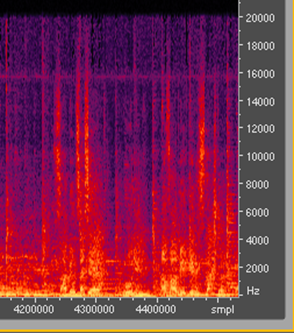
\includegraphics[width=0.3\textwidth]{pic-spectrogram-03}
\caption{Пример спектрограммы сигнала с шумом оборудования около 16 кГц}
\label{pic-spectrogram-03}
\end{figure}

\begin{figure}[h!]
\centering
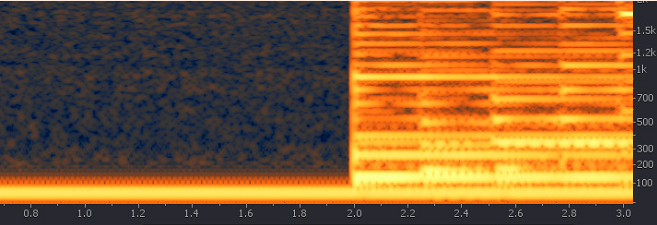
\includegraphics[width=0.5\textwidth]{pic-hum-01}
\caption{Пример спектрограммы сигнала с гулом 50 Гц}
\label{pic-hum-01}
\end{figure}

В некоторых случаях наводки от сети электрического тока и прочие шумы оборудования проникают в область высоких часотот из-за наличия высших гармоник, что воспринимается на слух как жужжание. На рис. \ref{pic-hum-02} приведен пример сигналограммы с тамим видом шума.

В отличие от гула и жужжания, шум шипения не сосредоточен на отдельных дискретных частотах. Шипение может иметь широкий спектр вплоть до всего частотного диапазона (рис. \ref{pic-hiss-01}). Такой вид шума могут создавать проигрыватели магнитных лент и кассет, шум вентилятора или системы кондиционирования. 

\begin{figure}[h!]
\centering
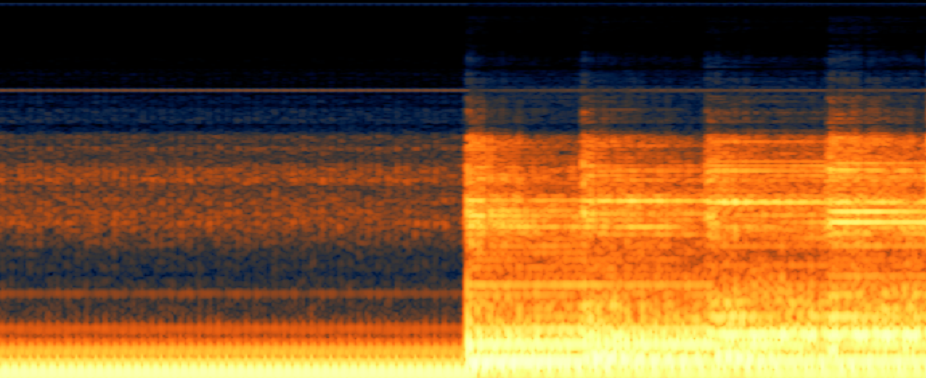
\includegraphics[width=0.5\textwidth]{pic-hum-02}
\caption{Пример спектрограммы сигнала с жужжанием}
\label{pic-hum-02}
\end{figure}

\begin{figure}[h!]
\centering
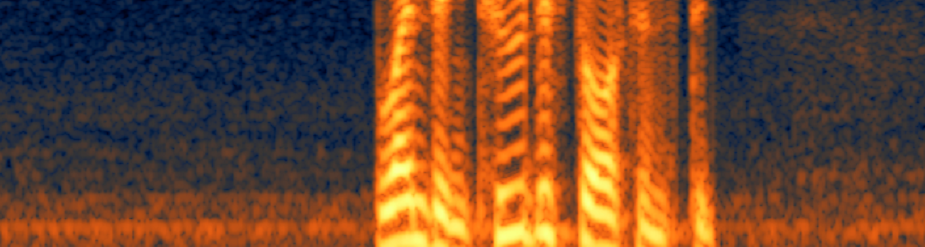
\includegraphics[width=0.5\textwidth]{pic-hiss-01}
\caption{Пример спектрограммы с шипением}
\label{pic-hiss-01}
\end{figure}

В записи могут присутствовать нерегулярные и непериодические шумы, имеющие различную природу и частотный состав: одни в чем-то похожи на шипение, другие~--- на гул. В качетве примера можно привести такие распространенные звуки, как кашель, чихание, шаги, гудок машины, звонок телефона и т.д. На рис. \ref{pic-ringing-01} представлен пример спектрограммы звука кашля, а на рис. \ref{pic-cough-01} ~--- пример спектрограммы телефонного звонка.

\begin{figure}[h!]
\centering
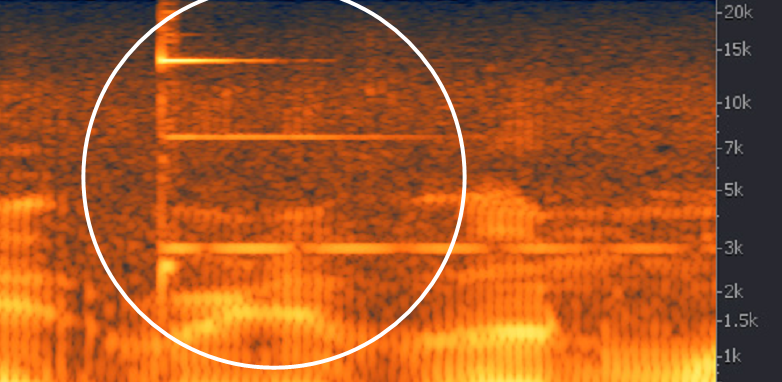
\includegraphics[width=0.5\textwidth]{pic-ringing-01}
\caption{Пример спектрограммы со звуком звонка}
\label{pic-ringing-01}
\end{figure}

\begin{figure}[h!]
\centering
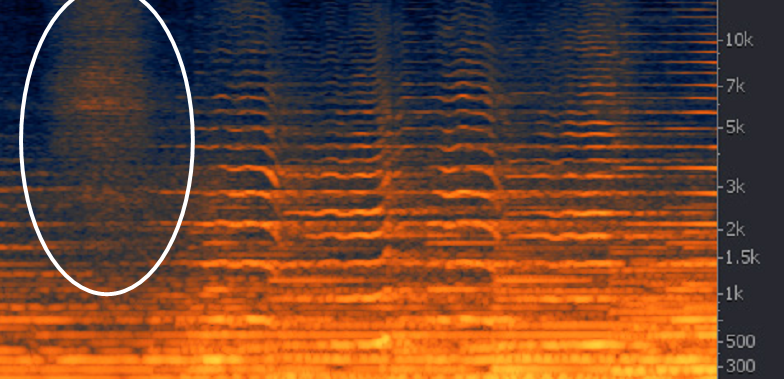
\includegraphics[width=0.5\textwidth]{pic-cough-01}
\caption{Пример спектрограммы со звуком кашля}
\label{pic-cough-01}
\end{figure}

\subsection{Амплитудно-частотный график спектра}
Командой \textit{Window > Frequency Analysis} открывается окно спектрального анализатора. При открытии окна происходит предварительный расчет спектра короткого фрагмента волновой формы, начало которого совпадает с позицией курсора. Если же выделен фрагмент волновой формы (или даже вся волновая форма), то рассчитывается средний спектр выделенной области.

\begin{figure}[h!]
\centering
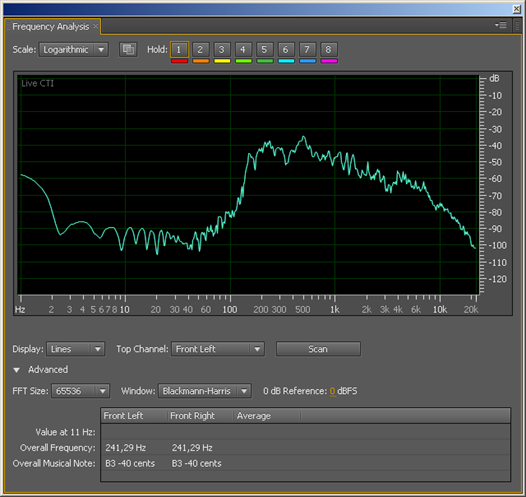
\includegraphics[width=0.45\textwidth]{pic-specter-01}
\caption{Окно графика амплитудно-частотного спектра}
\label{pic-specter-01}
\end{figure}

Если анализировать спектр в процессе воспроизведения волновой формы, то в окне \textit{Frequency Analysis} будет отображаться изменение значений мгновенного спектра. Расчет спектра производится раздельно для правого и левого каналов. 

Если в списке \textit{Scale} выбран элемент \textit{Linear}, то горизонтальная ось размечается в линейном масштабе. В линейном масштабе удобнее рассматривать весь спектр в целом, включая его высокочастотную область. Если выбран элемент \textit{Logarithmic}, то по горизонтали устанавливается логарифмический масштаб. Логарифмический масштаб позволяет наблюдать низкочастотную часть спектра в деталях. 

\begin{figure}[h!]
\centering
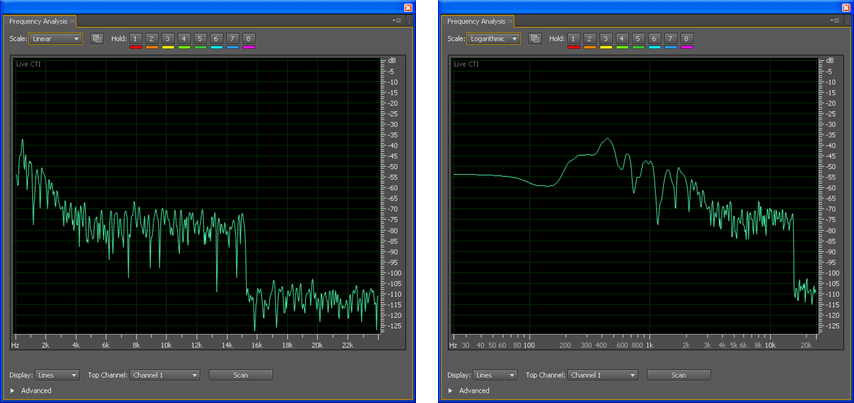
\includegraphics[width=0.90\textwidth]{pic-specter-02}
\caption{График спектра в линейном (слева) и логарифмическом (справа) масштабах}
\label{pic-specter-02}
\end{figure}

Для настройки детализации отображения спектра следует включить отображение дополнительных опций (кнопка \textit{Advanced}) и в списке \textit{FTT Size} выбрать размер выборки для расчета спектра. Чем больше значение, тем больше точность расчета спектра, но тем дольше расчет будет происходить.

\begin{figure}[h!]
\centering
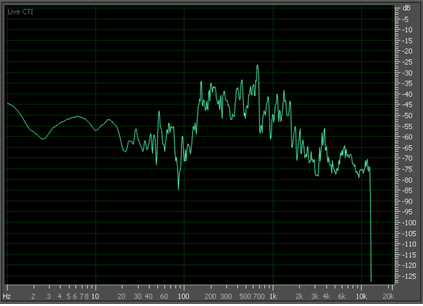
\includegraphics[width=0.5\textwidth]{pic-specter-03}
\caption{Пример график спектра сигнала}
\label{pic-specter-03}
\end{figure}

При анализе спектра следует обращать внимание на следующее:
\begin{itemize}
\item верхняя частота ограничения спектра (на рис. \ref{pic-specter-03}~--- около 13 кГц);
\item наличие наводок от сети переменного тока (частота 50Гц и ее нечетные гармоники);
\item наличие низкочастотного гула (подъем в области спектра ниже 100Гц, присутствует на рис. \ref{pic-specter-03}).
\end{itemize}

\subsection{Фазовый анализ}
\textit{Моносовместимость}~--- это свойство звукового файла, которое позволяет его прослушивать на монофоническом оборудовании. 

Несовместимость музыкальной композиции с монофоническим оборудованием появляется тогда, когда компоненты звукового сигнала левого и правого каналов оказываются в противофазе. Так как при преобразовании стерео сигнала в монофонический сигналы левого и правого каналов суммируются, то звуковые компоненты, находящиеся в противофазе, "<гасят"> друг друга, в результате чего возникают неприятные на слух искажения: партии некоторых инструментов могут вообще "<исчезнуть"> из композиции. В первую очередь это утверждение относится к партиям, панорамированным в центр. 

В компьютерной музыке такая ситуация является следствием применения специальных эффектов, изменяющих фазу звукового сигнала. 

\begin{figure}[h!]
\centering
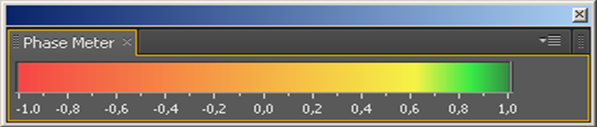
\includegraphics[width=0.5\textwidth]{pic-phase-01}
\caption{Панель измерителя фазы сигнала}
\label{pic-phase-01}
\end{figure}

Моносовместимость важна при передаче музыкальных композиций по радио и при сведении мультитрековой композиции. Определить на слух моносовместимость фонограммы без переключения в режим моно невозможно. 

В \textit{Adobe Audition} есть возможность контроля моносовместимости сигнала с помощью окна \textit{Phase Meter}, открываемого командой \textit{Window > Phase Meter}. Фонограмма является моносовместимой, если при проигрывании индикатор текущей фазы находится в зеленой зоне. Фонограмма мононесовместима, когда индикатор текущей фазы лежит в отрицательной области (от $-1.0$ до $0.0$).

\section{VST-инструменты анализа звука}

\textit{Virtual Studio Technology} (VST)~--- формат ресурсозависимых плагинов реального времени, которые подключаются к звуковым и музыкальным редакторам, секвенсорам и т. д.

VST-инструменты позволяют расширить функциональность программного обеспечения для обработки звука. Для подключения VST-инструментов и их использования в Adobe Audition необходимо:
\begin{enumerate}
\item Установить VST-инструмент (как правило, программой-установщиком).
\item Подключить VST-инструмент в \textit{Adobe Audition}.
\end{enumerate}

Подключение VST-инструмента осуществляется в окне, вызываемом командой \textit{Effects > Audio Plug-in Manager} (рис. \ref{pic-plugin-01}). 

\begin{figure}[h!]
\centering
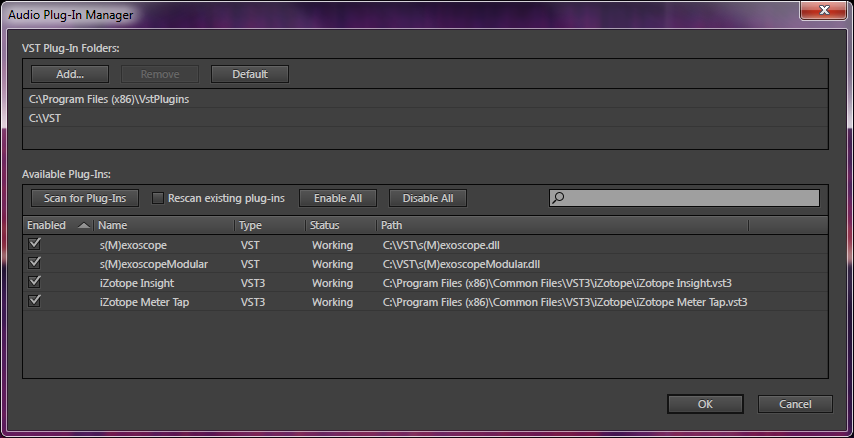
\includegraphics[width=0.75\textwidth]{pic-plugin-01}
\caption{Окно для поключения VST-инструментов}
\label{pic-plugin-01}
\end{figure}

В верхней части окна располагается список с именами каталогов, в котором будет осуществляться поиск файлов VST-инструментов. В нижней части отображается список инструментов, найденный \textit{Adobe Audition}. Для того, чтобы обновить список (после установок новых инструментов), необходимо нажать на кнопку "<\textit{Scan for Plug-Ins}">. Для подключения новых инструментов необходимо у соответствующего элемента списка установить флажок "<\textit{Enabled}"> и нажать кнопку "<ОК">.

После этого эффект или группа эффектов должны появиться либо в \textit{Adobe Audtion} в меню \textit{Effects > VST}, либо \textit{Effects > VST 3}.

\subsection{VST-инструмент s(M)exoscope}

Инструмент \textit{s(M)exoscope} является эффектом, реализующим цифровой осциллограф, который позволяет в режиме реального времени анализировать сигналлограмму и ее изменение под действием различных эффектов (рис. \ref{pic-exoscope-01}). 

\begin{figure}[h!]
\centering
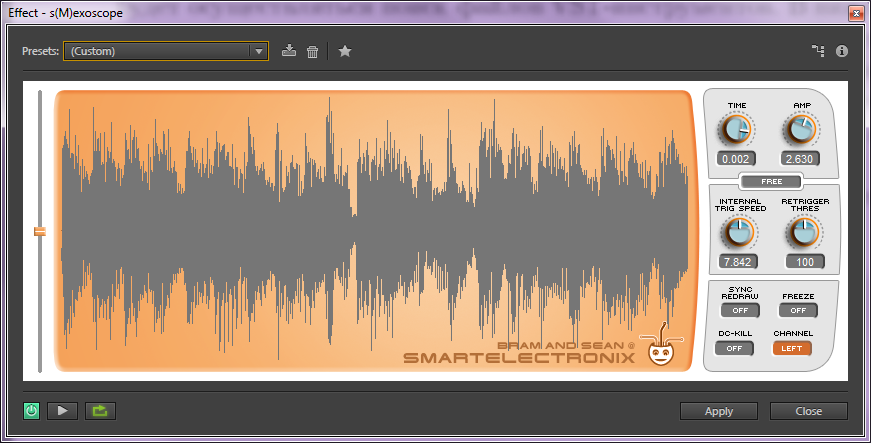
\includegraphics[width=0.75\textwidth]{pic-exoscope-01}
\caption{Окно эффекта s(M)exoscope}
\label{pic-exoscope-01}
\end{figure}

Параметр \textit{Time} задает количество точек для отображения одного цифрового отсчета. Например, значение 0.002 означает, что каждый пиксел будет отображать фрагмент длиной 500 отсчетов.

Параметр \textit{Amp} позволяет увеличить или уменьшить амплитуду сигналлограммы, например для того, чтобы сигнал уместился в окне полностью или не бы слишком маленьким.

Инструмент \textit{s(M)exoscope} имеет несолько режимов, отличающихся тем, как часто сигналограмма будет обновляться:
\begin{itemize}
\item \textit{Free}~--- обновление в режиме реального времени;
\item \textit{Internal}~--- обновление с частотой, заданной параметром \textit{Internal Trig Speed}. 
\item \textit{Rising}~--- обновление  будет происходить каждый раз, когда пик сигналлограммы превысит порог, заданный слайдером, расположенным в левой части окна эффекта;
\item \textit{Falling}~---обновление  будет происходить каждый раз, когда пик сигналлограммы станет ниже порога;
\end{itemize}

Для всех режимов параметр \textit{Retrigger Threshold} определяет, как часто могут следовать друг за другом два последовательных события обновления экрана. Например, если \textit{Retrigger Threshold}~$=450$, тогда экран не обновится, пока если между двумя событиями пройдет меньше 450 отсчетов. 

Если опция \textit{Sync Redraw} включена, то обновление экрана будет происходить в момент переполнения внутреннего буфера памяти эффекта. Опция \textit{Freeze} останавливает обновление экрана. При включенной опции \textit{DC-Kill} автоматически будет компенсироваться уровень постоянной составляющей сигнала. Параметр \textit{Channel} позволяет выбрать отображаемый канал (левый или правый).

\subsection{iZotope Insight}
VST-инструмент \textit{Insight} компании \textit{iZotope} (см. рис. \ref{pic-insight-01}) предназначен для проведения полноценного анализа звукового сигнала и предоставляет набор инструментов для измерения различных параметров сигнала, инструментов визуализации для просмотра изменений, которые происходят с сигналом в процессе микширования и мастеринга, для обнаружения различных проблем в сигнале и для того, чтобы итоговый сигнал соответствовал стандартам по громкости. 

\begin{figure}[h!]
\centering
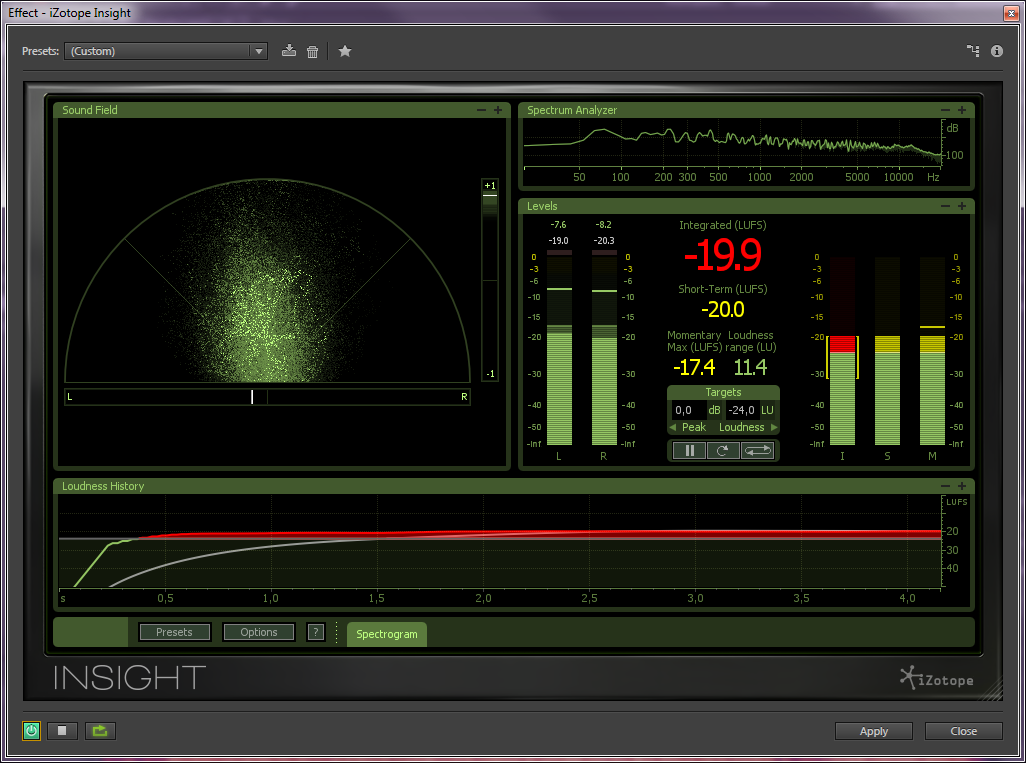
\includegraphics[width=0.75\textwidth]{pic-insight-01}
\caption{Окно эффекта \textit{iZotope Insight}}
\label{pic-insight-01}
\end{figure}

\textit{iZotope Insight} содержит следующие инструменты: 
\begin{itemize}
\item измеритель уровня сигнала;
\item измеритель громкости сигнала;
\item спектрограмма;
\item график амплитудно-частотного спектра;
\item анализатор фазы для двух- и многоканального звука;
\item график изменения громкости. 
\end{itemize} 

В нижней части окна эффекта (рис. \ref{pic-insight-02}) располагаются кнопки для открытия списка шаблонов настройки \textit{Presets}, нараметров настройки \textit{Options}, а также закладки тех инструментов, которые были скрыты в процессе работы с инструментом.

\begin{figure}[h!]
\centering

\includegraphics[width=0.75\textwidth]{pic-insight-02}
\caption{Нижняя часть окна эффекта iZotope Insight}
\label{pic-insight-02}
\end{figure}

Настройки (рис. \ref{pic-insight-03}) позволяют изменять параметры отображения отдельных инструментов и общие настройки эффекта, например, размер буфера памяти (влияющего на быстродействие эффекта).

\begin{figure}[h!]
\centering
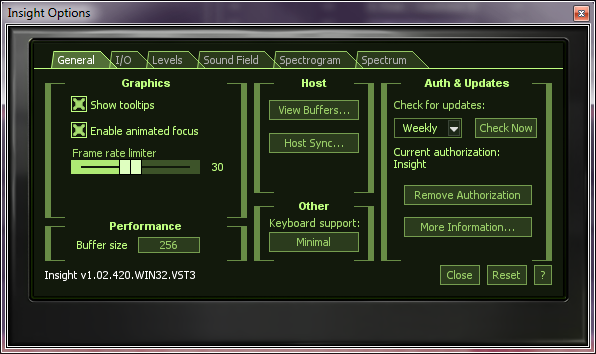
\includegraphics[width=0.75\textwidth]{pic-insight-03}
\caption{Окно настроек параметров эффекта \textit{iZotope Insight}}
\label{pic-insight-03}
\end{figure}

Рассмотрим основные инструменты эффекта \textit{iZotope Insight}.

\paragraph{Измерители уровня} (\textit{Level Meters}, рис. \ref{pic-insight-04}) позволяют осуществлять мониторинг уровня сигнала в отдельных каналах (левом и правом для стерео 2.0; L, R, C, Ls, Rs, Lfe~--- для шестиканального звука). 

\begin{figure}[h!]
\centering
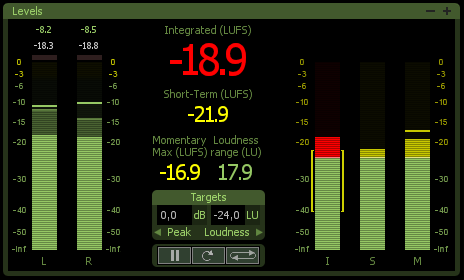
\includegraphics[width=0.75\textwidth]{pic-insight-04}
\caption{Измерители уровня сигнала}
\label{pic-insight-04}
\end{figure}

Инструмент \textit{Level Meters} отображает уровень сигнала, причем отображается одновременно и мгновенное значение (\textit{true-peak}) и уровень среднеквадратичной мощности (\textit{RMS, Root Mean Square}). Данный инструмент позволяет следить за изменением уровня сигнала с течением времени, а также обнаруживать клипирование сигнала.

\textit{Level Meters} позволяет измерять уровень сигнала следующими методами:
\begin{itemize}
\item \textit{Peak+RMS}~--- верхняя часть столбца соответствует измерению пиковой громкости сигнала, а нижняя и чуть более темная~--- среднеквадратичному уровню (рис. \ref{pic-insight-05}).
\item \textit{K-System}~--- метод измерения громкости звука с учетом прихоаккустических особенностей слуха человека. Существует несколько стандартных шкал: K-20, K-14, K-12, где за уровень 0 дБ приняты величины, соответственно, $-20$~дБ, $-14$~дБ и $-12$~дБ соответственно (рис. \ref{pic-insight-06}).
  \begin{itemize}
  	\item шкала K-12 используется для материала и небольшим динамическим диапазоном и подвергнутого сильной компрессии (например, для трансляции по радиоканалам);
  	\item шкала K-14 используется для материала со средней степенью компрессии: поп и рок-музыка, аудио для цифрового видео и т.п.
  	\item шкала K-20 используется для материала с большим динамическим диапазоном: запись концертного исполнения музыки, "<аудиофильские"> записи, классическая (симфоническая) музыка и аудио в формате шестиканального звука.
  \end{itemize}
\end{itemize}

\begin{figure}[h!]
\centering
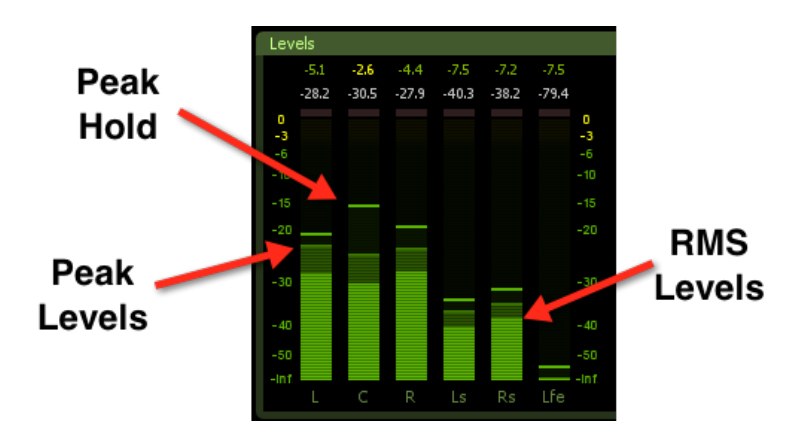
\includegraphics[width=0.75\textwidth]{pic-insight-05}
\caption{Peak и RMS-уровни сигнала}
\label{pic-insight-05}
\end{figure}

\begin{figure}[h!]
\centering
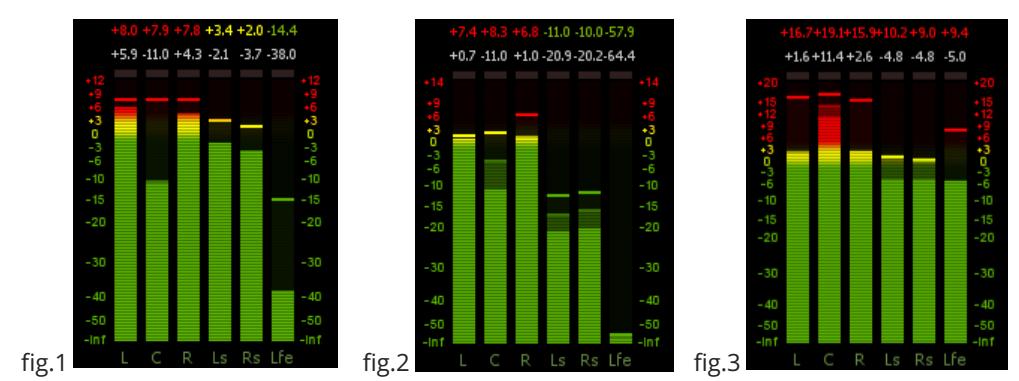
\includegraphics[width=0.75\textwidth]{pic-insight-06}
\caption{Пример отображения с использованием шкал K-20, K-14, K-12}
\label{pic-insight-06}
\end{figure}

\paragraph{Инструменты измерения громкости} (\textit{Loudness Meters}) осуществляют измерение громкости в соответствии с рекомендациями интернациональных стандартов \textit{International Telecommunication Union} (ITU-R BS.1770-1,2,3) и \textit{European Broadcasting Union} (EBU R128). 

Измерители уровня громкости в режиме реального времени рассчитывают и отображают воспринимаюмую человеком громкость аудио сигнала. Существуют следующие методы расчета громкости (рис. \ref{pic-insight-07}):
\begin{itemize}
\item мгновенная громкость (\textit{Momentary}): расчет громкости на интервале в 400~мс. Данное значение отображается в столбце с литерой "<M">. 
\item максимум мгновенной громкости (\textit{Momentary Max}): максимальное значение из всех рассчитанных значений мгновенной громкости за прошедший период времени; данное значение отображается в поле \textit{Momentary Max}. 
\item краткосрочная громкость (\textit{Short-term}): расчет громкости на интервале в 3~сек.  Данный параметр удобен для анализа тренда громкости сигнала и отображается в стоблце с литерой "<S">.
\item суммарная громкость (\textit{Integrated}): расчет громкости производится на бесконечном отрезке времени (т.е. фактически усредняется на всем времени сигнала). Данный параметр отображается в стоблце с литерой "<I"> и в одноименном поле.
\item динамический диапазон громкости (\textit{Loudness Range}): отношение максимальной к минимальной громкости сиганала на всем периоде его звучания, выражается в единицах громкости (\textit{Loudness Units}, \textit{LU}). 1~\textit{LU} равен 1~дБ.
\end{itemize}

\begin{figure}[h!]
\centering
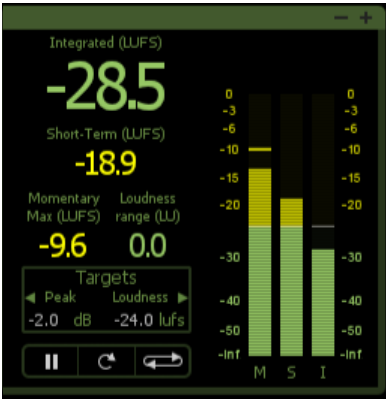
\includegraphics[width=0.4\textwidth]{pic-insight-07}
\caption{Индикаторы уровня громкости}
\label{pic-insight-07}
\end{figure}

График изменения громкости \textit{Loudness History Graph} позволяет выполнять мониторинг 
тренда изменения громкости на протяжении всего времени сигнала (рис. \ref{pic-insight-08}). На графике могут отображаться: краткосрочная громкость, моментальнная громкость и суммарная громкость, а также случаи превышения суммарной громкостью заданного порога (\textit{Loundness Target}).

Если данный инструмент развернуть на полный экран, то станут доступны кнопки настройки цвета графиков и кнопки копирования данных в графической форме и в форме таблицы значений.

\begin{figure}[h!]
\centering
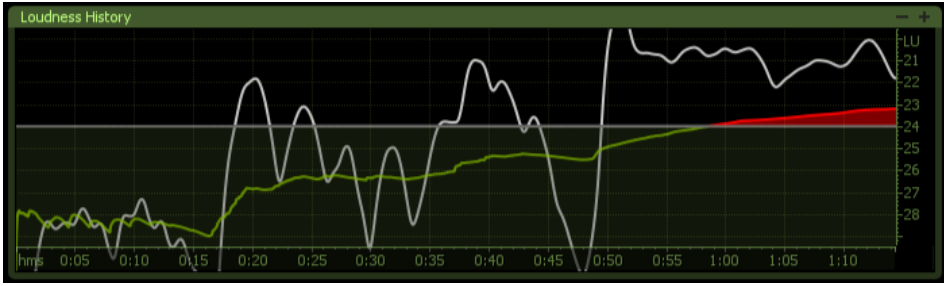
\includegraphics[width=0.75\textwidth]{pic-insight-08}
\caption{График изменения уровня громкости}
\label{pic-insight-08}
\end{figure}

\paragraph{Вектороскоп} (\textit{Vectorscope}) позволяет анализировать корреляцию между стереоканалами сигнала. \textit{Surround Scope}~--- вариант вектороскопа для анализа шестиканального звука.

Вектороскоп (рис. \ref{pic-insight-08}) позволяет анализировать различие между двумя каналами стерео сигнала при помощи графика в полярных координатах: полярный угол определяется разностью фаз каналов, а полярный радиус~--- суммой амплитуд каналов.  

\begin{figure}[h!]
\centering
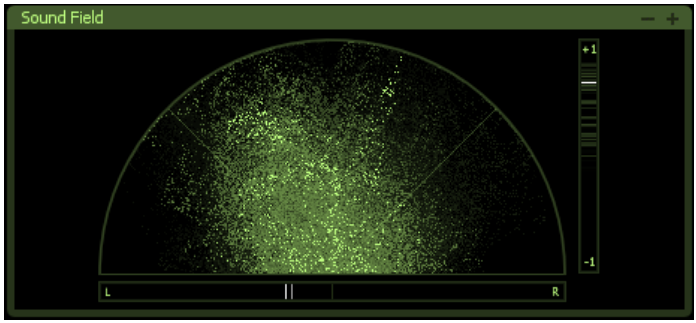
\includegraphics[width=0.75\textwidth]{pic-insight-09}
\caption{Пример вектороскопа}
\label{pic-insight-08}
\end{figure}

Моносигнал будет отображаться как вертикальная линия. Чем шире стерепанорама сигнала, тем более вытянутой вдоль горизонтальной оси будет отображаемый график. Если каналы будут в противофазе, то график на вектороскопе выйдет за границы линий, определяющих так называемую "<безопасную зону">. Если разница фаз между двумя каналами будет равняться $\pi$ (один из каналов является инверсией другого), то на вектороскопе будет отображаться горизонтальная линия.

Если сигнал будет иметь клипирование, то точки на вектороскопе будут окрашены в красный цвет.

Вектороскоп имеет несколько режимов отображения сигнала:
\begin{itemize}
\item отсчеты в полярных координатах (\textit{Polar Sample Vectorscope}, рис. \ref{pic-insight-08});
\item уровень каналов в полярных координатах (\textit{Polar Level Vectorscope}, рис. \ref{pic-insight-09});
\item в виде фигур Лиссажу (\textit{Lissajous Vectorscope}, рис. \ref{pic-insight-10});
\end{itemize}

В нижней части вектороскопа отображается измеритель фазы, а в правой~--- измеритель коэффициента корреляции каналов.

\begin{figure}[h!]
\centering
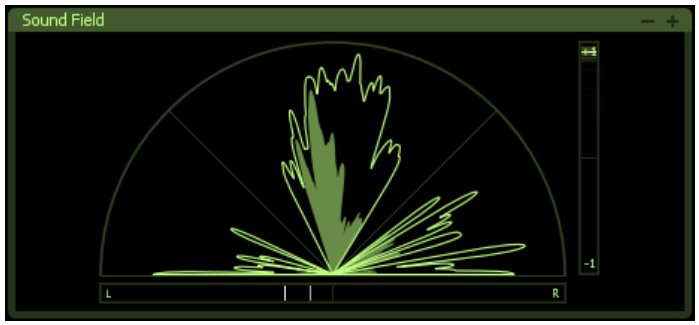
\includegraphics[width=0.75\textwidth]{pic-insight-10}
\caption{Вектороскоп в режиме Polar Level}
\label{pic-insight-09}
\end{figure}

\begin{figure}[h!]
\centering
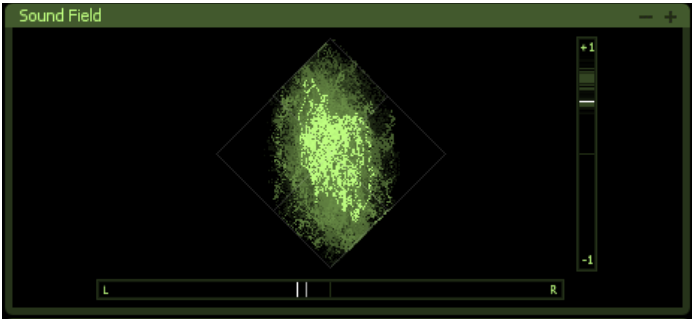
\includegraphics[width=0.75\textwidth]{pic-insight-11}
\caption{Вектороскоп в режиме Lissajous}
\label{pic-insight-10}
\end{figure}

\paragraph{Спектрограмма} (\textit{Spectrogram}). В эффекте \textit{iZotope Insight} спектрограмма может отображаться как в двумерном (рис. \ref{pic-insight-13}), так и в трехмерном виде (рис. \ref{pic-insight-12}) и поддерживает операции вращения и масштабирования. Для отображения спектрограммы видеокарта должна поддерживать \textit{Open~GL~2.0}.

\begin{figure}[h!]
\centering
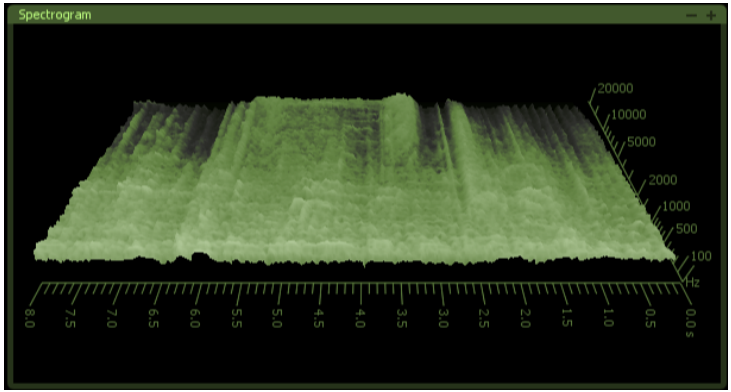
\includegraphics[width=0.75\textwidth]{pic-insight-12}
\caption{Пример спектрограммы в режиме 3D}
\label{pic-insight-12}
\end{figure}

\begin{figure}[h!]
\centering
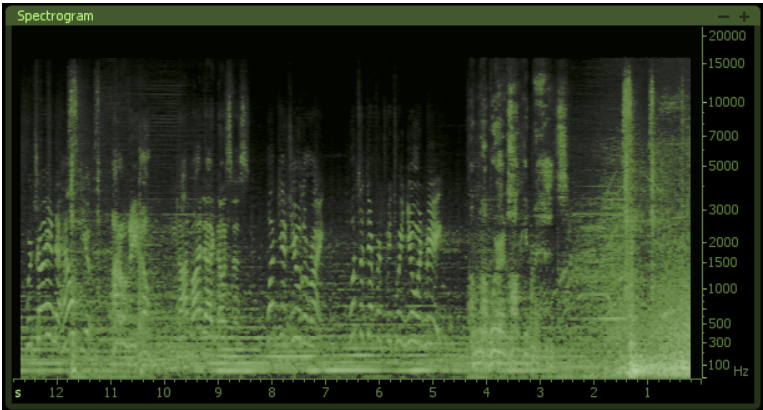
\includegraphics[width=0.75\textwidth]{pic-insight-13}
\caption{Пример спектрограммы в режиме 2D}
\label{pic-insight-13}
\end{figure}

\paragraph{Спектральный анализатор} (\textit{Spectrum Analyzer}). Классический график амплитудно-частотного спектра позволяет выполнять частотный анализ в режиме реального времени. График поддерживает масштабирование по обоим осям и может отображаться в следующих режимах:
\begin{itemize}
\item \textit{Linear}: в виде непрерывной линии (рис. \ref{pic-insight-14});
\item \textit{1/3 Octave}: в виде гистограммы с шириной полосы в $1/3$ октавы; 
\item \textit{Full Octave}: в виде гистограммы с шириной полосы в $1$ октаву;
\item \textit{Critical bands}: в виде гистограммы с переменной шириной полосы, соответствующей ширине критической полосы, равной $1$ Барк (рис. \ref{pic-insight-15}). 
\end{itemize}

\begin{figure}[h!]
\centering
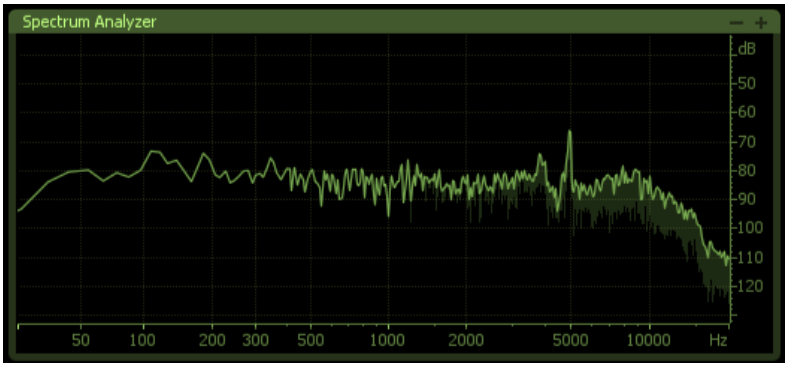
\includegraphics[width=0.75\textwidth]{pic-insight-14}
\caption{Пример графика спектра в режиме \textit{Linear}}
\label{pic-insight-14}
\end{figure}

\begin{figure}[h!]
\centering
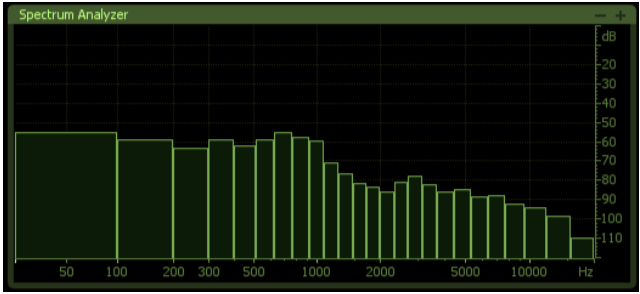
\includegraphics[width=0.75\textwidth]{pic-insight-15}
\caption{Пример графика спектра в режиме \textit{Critical bands}}
\label{pic-insight-15}
\end{figure}

\section*{Библиографический список}
\begin{enumerate}
\item Петелин Р.Ю., Петелин Ю.В.~Adobe Audition. Обработка звука для цифрового видео СПб: БХВ-Петербург, 2004. - 400~стр.
\item http://www.izotope.com
\item http://bram.smartelectronix.com/plugins.php?id=4
\end{enumerate}

\end{document}

